
\begin{figure}[H]
\centering
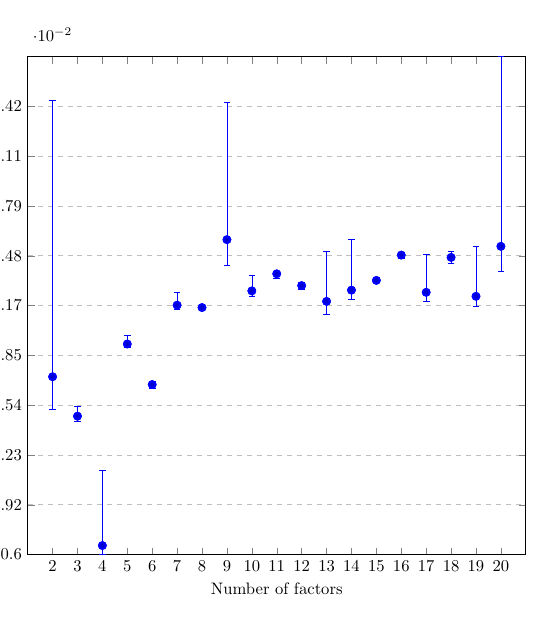
\begin{tikzpicture}[scale=0.6, trim axis left, trim axis right]
\begin{axis}[
    width=1\textwidth,
    height=1\textwidth,
    xlabel={Number of factors},
    ylabel={Time taken (s)},
    xmin=1.0, xmax=21.0,
    ymin=0.006036, ymax=0.037316,
    xticklabels={2, 3, 4, 5, 6, 7, 8, 9, 10, 11, 12, 13, 14, 15, 16, 17, 18, 19, 20},
    xtick={2, 3, 4, 5, 6, 7, 8, 9, 10, 11, 12, 13, 14, 15, 16, 17, 18, 19, 20},
    ytick={0.006036, 0.009164, 0.012292, 0.01542, 0.018548, 0.021676, 0.024804, 0.027932, 0.03106, 0.034188},
    ymajorgrids=true,
    grid style=dashed,
]

\addplot+[
    blue,
    very thick,
    forget plot,
    only marks
    ]
    plot[
    very thick,
    error bars/.cd,
    y dir=plus,
    y explicit
    ]
    table[x=x,y=y,y error expr=\thisrow{y-max}] {
    x    y    y-max
    11	0.0236688	0.0001792
10	0.0225958	0.0010052
13	0.0219352	0.0031238
12	0.0229276	0.0002124
15	0.0232545	0.0001765
14	0.0226425	0.0031865
17	0.0225047	0.0024053
16	0.0248437	0.0001843
19	0.0222563	0.0031077
18	0.0246986	0.0004024
20	0.0253932	0.0119228
3	0.0147288	0.0005922
2	0.0172045	0.0173345
5	0.0192603	0.0005587
4	0.0066054	0.0047186
7	0.0216986	0.0008004
6	0.0167151	0.0002099
9	0.0258125	0.0086195
8	0.0215497	0.0002093

    };

\addplot+[
    blue,
    very thick,
    forget plot,
    only marks
    ]
    plot[
    very thick,
    error bars/.cd,
    y dir=plus,
    y explicit
    ]
    table[x=x,y=y,y error expr=\thisrow{y-min}] {
    x    y    y-min
    11	0.0236688	-0.0002628
10	0.0225958	-0.0003488
13	0.0219352	-0.0008312
12	0.0229276	-0.0002046
15	0.0232545	-0.0001455
14	0.0226425	-0.0005675
17	0.0225047	-0.0005527
16	0.0248437	-0.0001877
19	0.0222563	-0.0006153
18	0.0246986	-0.0003486
20	0.0253932	-0.0015932
3	0.0147288	-0.0003158
2	0.0172045	-0.0020495
5	0.0192603	-0.0001813
4	0.0066054	-0.0005694
7	0.0216986	-0.0002826
6	0.0167151	-0.0002121
9	0.0258125	-0.0016305
8	0.0215497	-0.0001557

    };

\end{axis}
\end{tikzpicture}
\vspace{-0.3cm}
\caption{Medium primes}\label{fig:TrialDivisionmediumprimesfactors}
\end{figure}
